%------------------Ejercicio 1--------------------------------

\begin{question}
  Sea  $S$  la superficie dada por $x^{2}+ y^{2} = z$ con $z \geq 2$  y $x^{2}+ y^{2} \leq 9.$  Calcular el \'area de $S.$
\end{question}

%------------------Ejercicio 2--------------------------------

\begin{question}
  Sea $C$ la curva simple definida por la intersecci\'on de las superficies $x^{2}+z^{2}=16$,  $y+z=4$ con $y\leq 4$ y sea $g$ una funci\'on escalar $C^{1}(\mathbb{R})$. Calcular la integral sobre $C$ del campo $\mathbf{F}(x,y,z)=(x,\;g(y),\;g(z)).$ Indicar la orientaci\'on elegida.
\end{question}

%------------------Ejercicio 3--------------------------------

\begin{question}
  Sean $\mathbf{F}(x,y,z)=(-xy+yz,\;-y^{2}+xz,\; xz)$, $a \in \mathbb{R}$ positivo  y $S$ la superficie de seis caras que encierra el cuerpo dado por $0\leq x \leq  a$, $0 \leq  y \leq  a $ y  $0 \leq  z \leq a$ orientada con normales exteriores.   Hallar $a$ de manera que el flujo de $\mathbf{F}$ a trav\'es  de $S$ sin su cara superior sea $-24$.
\end{question}

%------------------Ejercicio 4--------------------------------

\begin{question}
  Calcule la masa del cuerpo definido por $z\leq \sqrt{x^{2} + y^{2} }$,  $x^{2} + y^{2} + z^{2} \leq 32$,  en el primer octante, si su densidad es proporcional a la distancia de un  punto al plano $z=0.$
\end{question}

\newpage

%------------------Solucion 1--------------------------------

\begin{solution}
  $S$ es una secci\'on de paraboloide, como se puede observar en el siguiente gr\'afico.

  \begin{center}
    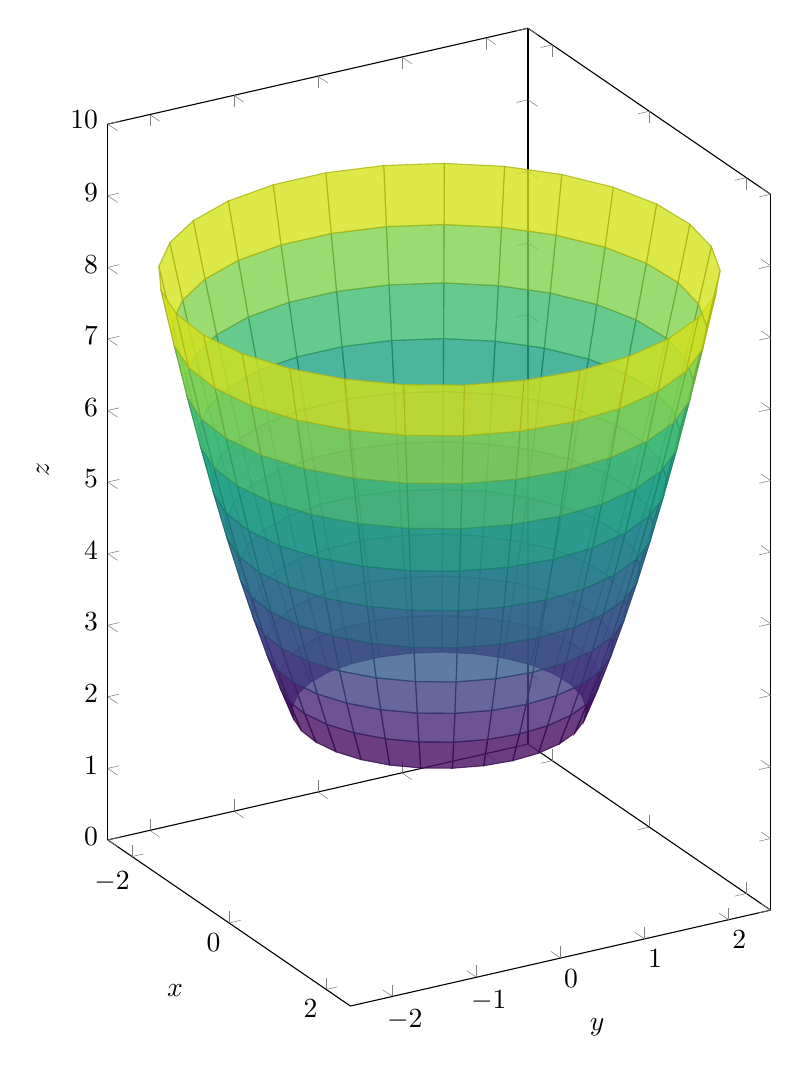
\begin{tikzpicture}
      \begin{axis}[
          view={60}{15},
          xlabel=$x$,
          ylabel=$y$,
          zlabel=$z$,
          xmin=-2.5,
          ymin=-2.5,
          zmin=0,
          xmax=2.5,
          ymax=2.5,
          zmax=10,
          samples=30,
          width=10cm,
          height=14cm,
          colormap/viridis,
        ]
        \addplot3 [surf, opacity=0.8, draw=none, restrict z to domain=2:9,
          data cs=polar, domain=0:360, y domain=0:4] (x, y, y^2);
      \end{axis}
    \end{tikzpicture}
  \end{center}

  Escribimos el conjunto $S$ como
  \[
    S=\{(x,y,z)\in \Re^3: x^2+y^2=z;\;2\leq z\leq 9 \}.
  \]
  Queremos calcular \[ \textcolor{red}{A}(S) = \iint_S dA.\]
  Para ello necesitaremos una parametrizaci\'on de $S$. Sea
  $$D=\{(\rho, \phi) \in\Re^2:    \sqrt{2}\leq \rho \leq 3;\;0\leq  \phi \leq 2\pi \}$$  y  sea  $$\boldsymbol{\Sigma}:D \subset\Re^2\to\Re^3  \mbox{ tal que }   \boldsymbol{\Sigma}(\rho, \phi)=(\rho \cos\phi, \rho \sen\phi , \rho^{2}).$$

  Primero calculamos las derivadas parciales de la parametrizaci\'on.
  \begin{align*}
    \boldsymbol{\Sigma}_{\rho} & =(\cos \phi,\;\sen \phi,\; 2\rho)         \\
    \boldsymbol{\Sigma}_\phi   & =(  -\rho \sen \phi,\;\rho \cos \phi,\;0)
  \end{align*}
  Entonces
  $$
    \boldsymbol{\Sigma}_{\rho} \times\boldsymbol{\Sigma}_\phi =
    (-2\rho^2 \cos\phi  , \;-2\rho^2 \sen \phi, \;\rho),
  $$
  $$\|  \boldsymbol{\Sigma}_{\rho} \times\boldsymbol{\Sigma}_\phi\|
    = \rho\sqrt{4\rho^2+1}.$$
  Quedando
  \begin{equation}
    \iint_S dA
    = \int_0^{2\pi} \int_{\sqrt{2}}^3 \|\boldsymbol{\Sigma}_{\rho}
    \times\boldsymbol{\Sigma}_\phi \| \; d\rho d\phi
    = \int_0^{2\pi} \int_{\sqrt{2}}^3 \rho\sqrt{4\rho^2+1}\;d\rho d\phi,
    \label{eq:integral1}
  \end{equation}
  \begin{gather*}
  u=4\rho^2+1 \rightarrow du = 8\rho\;d\rho, 
  \\[.2cm]
  = \frac{1}{8}\int_0^{2\pi} \int_9^{37} \sqrt{u}\;du d\phi
  = \frac{2\pi}{8}\frac{u^{\frac{3}{2}}}{\frac{3}{2}}\Bigg|_9^{37}
  = \frac{\pi}{4\cdot\frac{3}{2}} (37^{\frac{3}{2}} - 9^{\frac{3}{2}}) 
  \\[.2cm]
  = \frac{\pi}{6} (\sqrt{37^3} - \sqrt{9^3}).
  \end{gather*}
\end{solution}

%------------------Solucion 2--------------------------------

\begin{solution} 
La curva de la intersecci\'on se muestra en el siguiente gr\'afico.

\begin{center}
  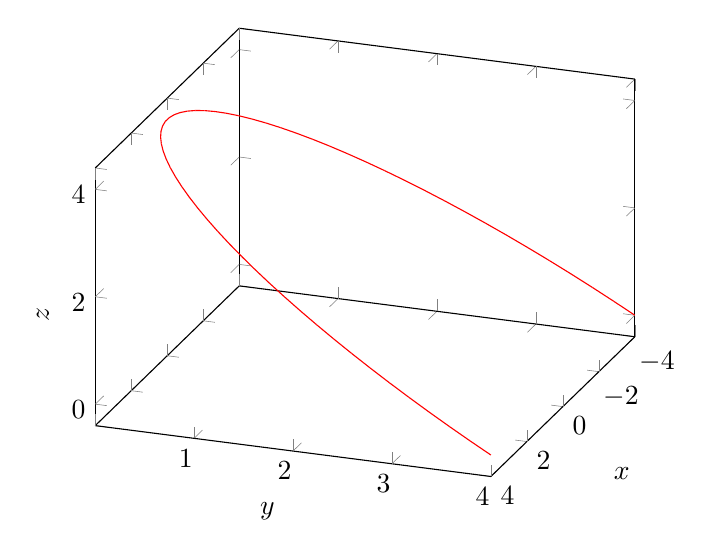
\begin{tikzpicture}
    \begin{axis}
        [view={110}{30},xlabel=$x$, ylabel=$y$, zlabel=$z$]
    \addplot3[
        domain=0:pi,
        samples = 60,
        samples y=0,
        mesh,
        color=red,
    ]
    ({4*cos(deg(x))},
    {-4*sin(deg(x))+4},
    {4*sin(deg(x))});
    \end{axis}
  \end{tikzpicture}
\end{center}

  Notemos que $C$ es una curva no cerrada. Para cerrarla, llamemos $C=C_1$, 
  $C_2=\{(x,y,z)\in\Re^3:z=0\;\land\;y=4\;\land\;|x|\leq4\}$, en palabras, $C_2$ es la recta que une la curva; y $C_0=C_1+C_2$. Y sea $\text{int}(C_0)=D$. Ahora $C_0$ es una curva simple cerrada. Entonces podemos aplicar el teorema de Stokes, eligiendo la orientaci\'on de $C_0$ tal que se cumpla la regla de la mano derecha.
  \[
      \oint_{C_0}\mathbf{F}\cdot d\mathbf{s}= \int_{C_1}\mathbf{F}\cdot d\mathbf{s} + \int_{C_2}\mathbf{F}\cdot d\mathbf{s} = \iint_D \nabla\times\mathbf{F}\cdot d\mathbf{A},
  \]
  ya que $\mathbf{F}$ es $C^1(\Re)$, pues sus componentes son $C^1(\Re)$, y $D\in\text{dom}(\mathbf{F})$.
  Notemos que $\nabla\times\mathbf{F}\equiv0\implies$
  \[
     \int_{C_1}\mathbf{F}\cdot d\mathbf{s} =- \int_{C_2}\mathbf{F}\cdot d\mathbf{s}.
  \]
  Ahora busquemos una trayectoria de $C_2$ que respete su orientaci\'on. Sea $\boldsymbol{\sigma}:[-4,4]\rightarrow\Re^3$
  tal que $\boldsymbol{\sigma}(t)=(t,4,0)$. Entonces $\boldsymbol{\sigma}'(t)=(1,0,0)$. Luego la integral de curva de $C_2$ es
  \begin{gather*}
    \int_{C_2}\mathbf{F}\cdot d\mathbf{s}
    =\int_{-4}^4 (\mathbf{F}\circ\boldsymbol{\sigma})\cdot\boldsymbol{\sigma}'\:dt
    =\int_{-4}^4 t\:dt = 0.
  \end{gather*}
  $\therefore$ la integral sobre la curva original $C=C_1$ es tambi\'en 0.
\end{solution}

%------------------Solucion 3--------------------------------

\begin{solution}
  Llamemos $\Omega$ al volumen que encierra $S$ y sea $S'$ la superficie de la cara superior de $S$, por lo que $S'$ tiene orientaci\'on igual que la tapa de $S$. En los siguientes gr\'aficos se puede ver la representaci\'on de $S$ y $S'$ respectivamente.

  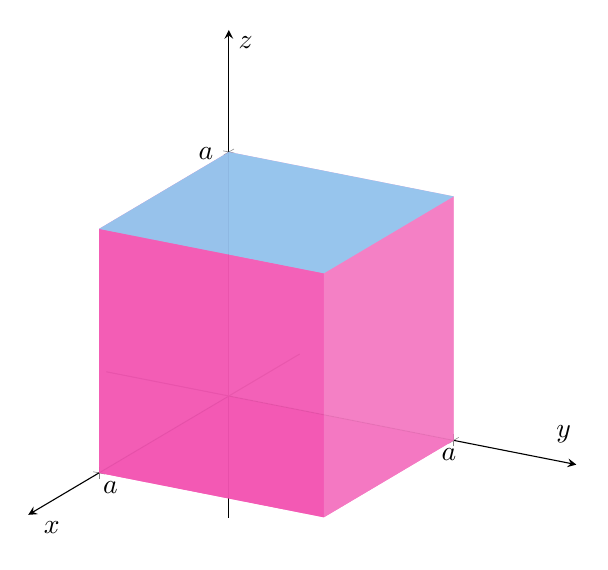
\begin{tikzpicture}
    \begin{axis}[
        axis equal,
        axis lines = center,
        height = 11cm, width = 11cm,
        view={120}{20},
        xlabel={$x$},
        ylabel={$y$},
        zlabel={$z$},
        zmin = -1, zmax = 3,
        xmin = -1, xmax = 3,
        ymin = -1, ymax = 3,
        xtick = {0, 2},
        xticklabels = {$0$, $a$},
        ytick = {0, 2},
        yticklabels = {$0$, $a$},
        ztick = {0, 2},
        zticklabels = {$0$, $a$},
        xlabel style={at={(axis cs:3,0,0)}, anchor=north west},
        xticklabel style={anchor=north west},
        ylabel style={at={(axis cs:0,3.1,0.05)}},
        yticklabel style={at={(axis cs:0,2,0)}},
      ]

      \addplot3[fill=magenta!80, opacity=0.8, draw=none] coordinates {(0,0,0) (0,2,0) (2,2,0) (2,0,0) (0,0,0)};
      \addplot3[fill=magenta!70, opacity=0.8, draw=none] coordinates {(0,0,0) (0,0,2) (2,0,2) (2,0,0) (0,0,0)};
      \addplot3[fill=magenta!60, opacity=0.8, draw=none] coordinates {(0,0,0) (0,2,0) (0,2,2) (0,0,2) (0,0,0)};
      \addplot3[fill=magenta!65, opacity=0.8, draw=none] coordinates {(2,0,0) (2,2,0) (2,2,2) (2,0,2) (2,0,0)};
      \addplot3[fill=magenta!50, opacity=0.8, draw=none] coordinates {(0,2,0) (0,2,2) (2,2,2) (2,2,0) (0,2,0)};
      \addplot3[fill=cyan!50, opacity=0.8, draw=none] coordinates {(0,0,2) (0,2,2) (2,2,2) (2,0,2) (0,0,2)};
    \end{axis}
  \end{tikzpicture}
  \hfill
  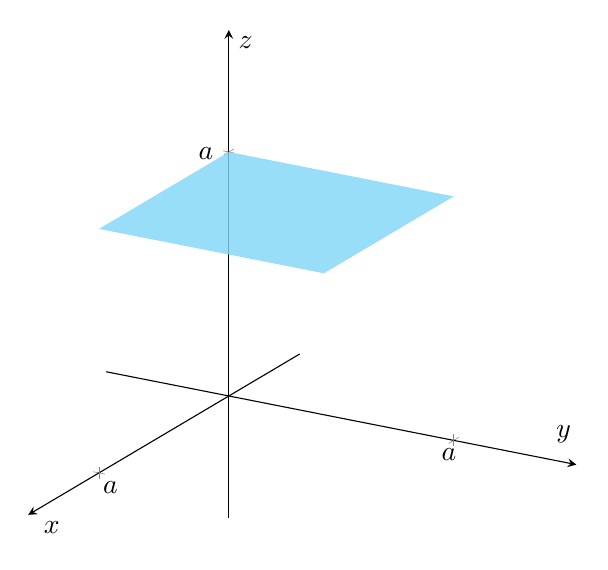
\begin{tikzpicture}
    \begin{axis}[
        axis equal,
        axis lines = center,
        height = 11cm, width = 11cm,
        view={120}{20},
        xlabel={$x$},
        ylabel={$y$},
        zlabel={$z$},
        zmin = -1, zmax = 3,
        xmin = -1, xmax = 3,
        ymin = -1, ymax = 3,
        xtick = {0, 2},
        xticklabels = {$0$, $a$},
        ytick = {0, 2},
        yticklabels = {$0$, $a$},
        ztick = {0, 2},
        zticklabels = {$0$, $a$},
        xlabel style={at={(axis cs:3,0,0)}, anchor=north west},
        xticklabel style={anchor=north west},
        ylabel style={at={(axis cs:0,3.1,0.05)}},
        yticklabel style={at={(axis cs:0,2,0)}},
      ]
      \addplot3[fill=cyan!50, opacity=0.8, draw=none] coordinates {(0,0,2) (0,2,2) (2,2,2) (2,0,2) (0,0,2)};
    \end{axis}
  \end{tikzpicture}


  Por el teorema de la divergencia tenemos que
  \[
    \iint_S \mathbf{F}\cdot d\mathbf{A}=\iiint_\Omega \nabla \cdot \mathbf{F}\;dV.
  \]
  Entonces la integral de flujo que buscamos es
  \[
    \iint_S \mathbf{F}\cdot d\mathbf{A} - \iint_{S'} \mathbf{F}\cdot d\mathbf{A}=
    \iiint_\Omega \nabla \cdot \mathbf{F}\;dV - \iint_{S'} \mathbf{F}\cdot d\mathbf{A}=-24.
  \]
  Primero calculamos el t\'ermino con la divergencia de $\mathbf{F}$.
  \[
    \nabla\cdot\mathbf{F}=-y-2y+x=x-3y
  \]
  \begin{gather*}
    \implies\iiint_\Omega\nabla\cdot\mathbf{F}\;dV=\int_0^a \int_0^a \int_0^a x-3y\;dxdydz\\[.2cm]
    \iff a\int_0^a \left(\frac{x^2}{2}-3yx\right)\Bigg|_0^a\;dy=a\int_0^a \frac{a^2}{2}-3ya\;dy\\[.2cm]
    \iff a\left( \frac{a^2}{2}y-3a\frac{y^2}{2} \right)=\frac{a^4}{2}-3\frac{a^4}{2}=-a^4
  \end{gather*}
  Segundo, el flujo sobre la tapa. Sea $\boldsymbol{\Sigma} : D\subset\Re^2\to S'\subset\Re^3$, una paremetrizaci\'on de $S'$ tal que $\boldsymbol{\Sigma}(u,v)=(u,v,a)$. Donde $D = \{(u,v)\in\Re^2:0\leq u\leq a;\;0\leq v \leq a\}$. Entonces
  \[
    \iint_{S'} \mathbf{F}\cdot d\mathbf{A}=\iint_D \mathbf{F}\circ\boldsymbol{\Sigma} \cdot (\boldsymbol{\Sigma}_u\times\boldsymbol{\Sigma}_v)\;dA.
  \]
  $\boldsymbol{\Sigma}_u=(1,0,0)$ y $\boldsymbol{\Sigma}_v=(0,1,0)$ $\implies \boldsymbol{\Sigma}_u\times\boldsymbol{\Sigma}_v=(0,0,1)=\boldsymbol{\eta}$. Por lo que $\boldsymbol{\Sigma}$ respeta la orientaci\'on de $S'$. Y $\mathbf{F}\circ\boldsymbol{\Sigma}=(-uv+va,\;-v^2+ua,\;ua) \implies \mathbf{F}\circ\boldsymbol{\Sigma}\cdot\boldsymbol{\eta}=ua$. Por lo tanto
  \[
    \iint_{S'} \mathbf{F}\cdot d\mathbf{A}=\int_0^a\int_0^a au\;dudv=a^2\frac{a^2}{2}=\frac{a^4}{2}.
  \]
  \[
    \therefore -a^4-\frac{a^4}{2}=-24\iff \frac{3}{2}a^4=24\iff a^4=16 \iff a=2.
  \]

\end{solution}

%------------------Solucion 4--------------------------------

\begin{solution}
  La distancia $d$ de un punto $(x_0,y_0,z_0)$ en el primer octante a el plano $z=0$ est\'a dada por $$d\Big(  (x_0,y_0,z_0); (x_0,y_0, 0) \Big)= \sqrt{(x_0-x_0)^2+(y_0-y_0)^2+z_0^2}=z_0.$$ Luego  la funci\'on de densidad del s\'olido es $\delta(z)=kz$,  con $k\in\Re$. Adem\'as  sea $$\Omega=\{(x,y,z)\in\Re^3:z\leq\sqrt{x^2+y^2}\:\land\:x^2+y^2+z^2\leq32\:\land\: x,y,z\geq0\}.$$
  Trabajaremos  en coordenadas esf\'ericas.  En este sentido,  recordemos lo siguiente.
  \[
    \begin{dcases}
      x=\rho\sen\phi\cos\theta \\
      y=\rho\sen\phi\sen\theta \\
      z=\rho\cos\phi
    \end{dcases}
  \]
  Por las condiciones de $\Omega$ tenemos que
  $$z\leq\sqrt{x^2+y^2}\iff\rho\cos\phi\leq\sqrt{\rho^2\sen^2\phi}=\rho |\sen\phi|.$$
  Adem\'as, como estamos en el primer octante,  nos queda que $\frac{\pi}{4} \leq\phi\leq\frac{\pi}{2}$ y  $0\leq\theta\leq\frac{\pi}{2}.$
  Por otro lado,  $$ \rho^2\leq32  \; \land \;  \rho \geq 0 \iff     0\leq  \rho\leq\sqrt{32}= 4 \sqrt{2}.$$
  Escribimos nuestro nuevo volumen $\Omega^*$  y usamos el teorema de cambio de variables.
  \[
    \Omega^*=\{(\rho,\phi,\theta)\in\Re^3:0\leq\rho\leq4\sqrt{2}\:\land\:0\leq\phi\leq\frac{\pi}{4}\:\land\:0\leq\theta\leq\frac{\pi}{2}\}
  \]
  Y la masa del s\'olido $\Omega$ queda
  \begin{align*}
    M & =\iiint_{\Omega^*}k\delta(z)\rho^2\sen\phi\:dV=\iiint_{\Omega^*}k\rho\cos\phi\rho^2\sen\phi\:d\rho d\phi d\theta \\
      & =k\int_0^{\frac{\pi}{2}} \int_0^{\frac{\pi}{4}} \int_0^{4\sqrt{2}}\rho^3\cos\phi\sen\phi \:d\rho d\phi d\theta   \\
      & =k2\pi\int_0^{\frac{\pi}{4}}\cos\phi\sen\phi\:d\phi\int_0^{4\sqrt{2}}\rho^3\:d\rho                               \\
      & =k2\pi\frac{1}{4}256=128k\pi.
  \end{align*}

\end{solution}